\setcounter{section}{53}

\section{Формальные степенные ряды, операции над ними. Определение обратного ряда. Критерий обратимости ряда (задача 13.5). Примеры нахождения обратных рядов (задача 13.6).}
\textbf{Формальный степенной ряд (ФСР)} — формальное алгебраическое выражение вида: $F=\sum_{i=0}^{\infty} a_{i}x^i$, где коэффициенты $a_i$ берутся из некоторого кольца $R$

\subsection*{Операции с ФСР:}
\begin{enumerate}
    \item сложение: $(a_0, a_1, ...)+(b_0, b_1, ...)=(a_0+b_0, a_1+b_1, ...)$
    \item умножение: \((a_0, a_1, ...)*(b_0, b_1, ...)=(..., \sum_{i=0}^{\infty} a_i b_{n-i}, ...)\)
    \item деление: $\frac{A}{B} = C \Leftrightarrow A=B*C$
    \item взятие производной: $(a_0, a_1, ...)'=(a_1, 2a_2, 3a_3, ...)$ (на лекции не было, но рассматривалось на семинаре)
\end{enumerate}

Формальный степенной ряд $A$ называется \textbf{обратимым}, если существует ряд $B$, такой что $A*B=(1, 0, 0, ...)$, а ряд $B$ называется \textbf{обратным} к ряду $A$.

\textbf{Критерий обратимости ряда}: ряд $(a_0, a_1, ...)$ обратим $\Leftrightarrow$  $a_0$ обратим в кольце $R$

$\blacktriangle$ $\Rightarrow$ Пусть ряд $A$ обратим и $B$ - обратный. Так как $A*B=(1, 0, ...)$, то $b_0 = \frac{1}{a_0}$ $\Rightarrow$ $a_0$ обратим

$\Leftarrow$ Начнем искать коэффициенты обратного ряда

\[b_0 = \frac{1}{a_0}\]

\[b_n = -\frac{1}{a_0} \sum_{i=0}^{n} a_i b_{n-i}, \forall n \geq 1\]

Следовательно, так как элемент $a_0$ обратим, такой ряд существует $\blacksquare$
\subsection*{Примеры нахождения обратных рядов}
\begin{enumerate}
    \item $\frac{1}{1-t}$
    \par $(1-t)(1-t)^{-1}=(1, 0, ...), (1-t)=(1, -1, 0, ...)$
    \par $a_0 b_0 = 1 \Rightarrow b_0=\frac{1}{a_0}=1$
    \par $a_0 b_1+b_0 a_1=0 \Rightarrow b_1=-\frac{a_1 b_0}{a_0}=1$
    \par $a_0 b_k + a_1 b_{k-1}=0 \Rightarrow b_k=-\frac{a_1 b_{k-1}}{a_0}=b_{k-1}=1$
    \par \textbf{Ответ:} $\frac{1}{1-t}=(1, 1, 1, ...)$
    \item $\frac{1}{(1-t)^2}$
    \par \textbf{I способ:} $\frac{1}{(1-t)^2}=(\frac{1}{1-t})^2$
    \par $(1-t)(1-t)=(1, 1, ...)(1, 1, ...)=(1, 2, 3, 4, ...)$
    \par \textbf{II способ (через формальную производную):} Заметим, что $(\frac{1}{(1-t)})'=\frac{1}{(1-t)^2}=(1, 2, 3, ...)$. В принципе, такое взятие производной согласуется с введенными операциями, так что можно написать и так. Но можем доказать это иначе.
    \par Продифференциируем выражение $(1-t) \frac{1}{(1-t)}=1$
    \par $(1-t)'\frac{1}{(1-t)} + (\frac{1}{1-t})'(1-t)=0$ (формула производной произведения доказывалась на семинаре просто через равенство коэффициентов)
    \par $\frac{1}{1-t}=(1-t)(\frac{1}{1-t})'$
    \par $\frac{1}{(1-t)^2}=(\frac{1}{1-t})'$
    \par \textbf{Ответ:} $\frac{1}{(1-t)^2}=(1, 2, 3, 4, ...)$
    \item $\frac{1}{(1-t)^m}$
    \par По аналогии с I способом пункта 2: 
    $$\frac{1}{(1-t)^m} = \underbrace{(1+t+t^2+...)...(1+t+t^2+...)}_{m раз}$$
    \par Заметим, что коэффициент при $x^i$ равен количеству неупорядоченных разбиений числа $i$ на ровно $m$ слагаемых. Таким образом $i$-ый коэффициент ряда имеет вид $C^{i}_{m+i-1}$
    \par \textbf{Ответ:} $(..., C^{i}_{m+i-1}, ...)$
\end{enumerate}

\section{Формальные степенные ряды, операции над ними. Определение обратного ряда. Пример деления в столбик. Комбинаторное тождество, получаемое с использованием формального степенного ряда $(\frac{1}{1-x^2})^2$}
\subsection*{Пример деления в столбик:}
\begin{figure}[h]
\center{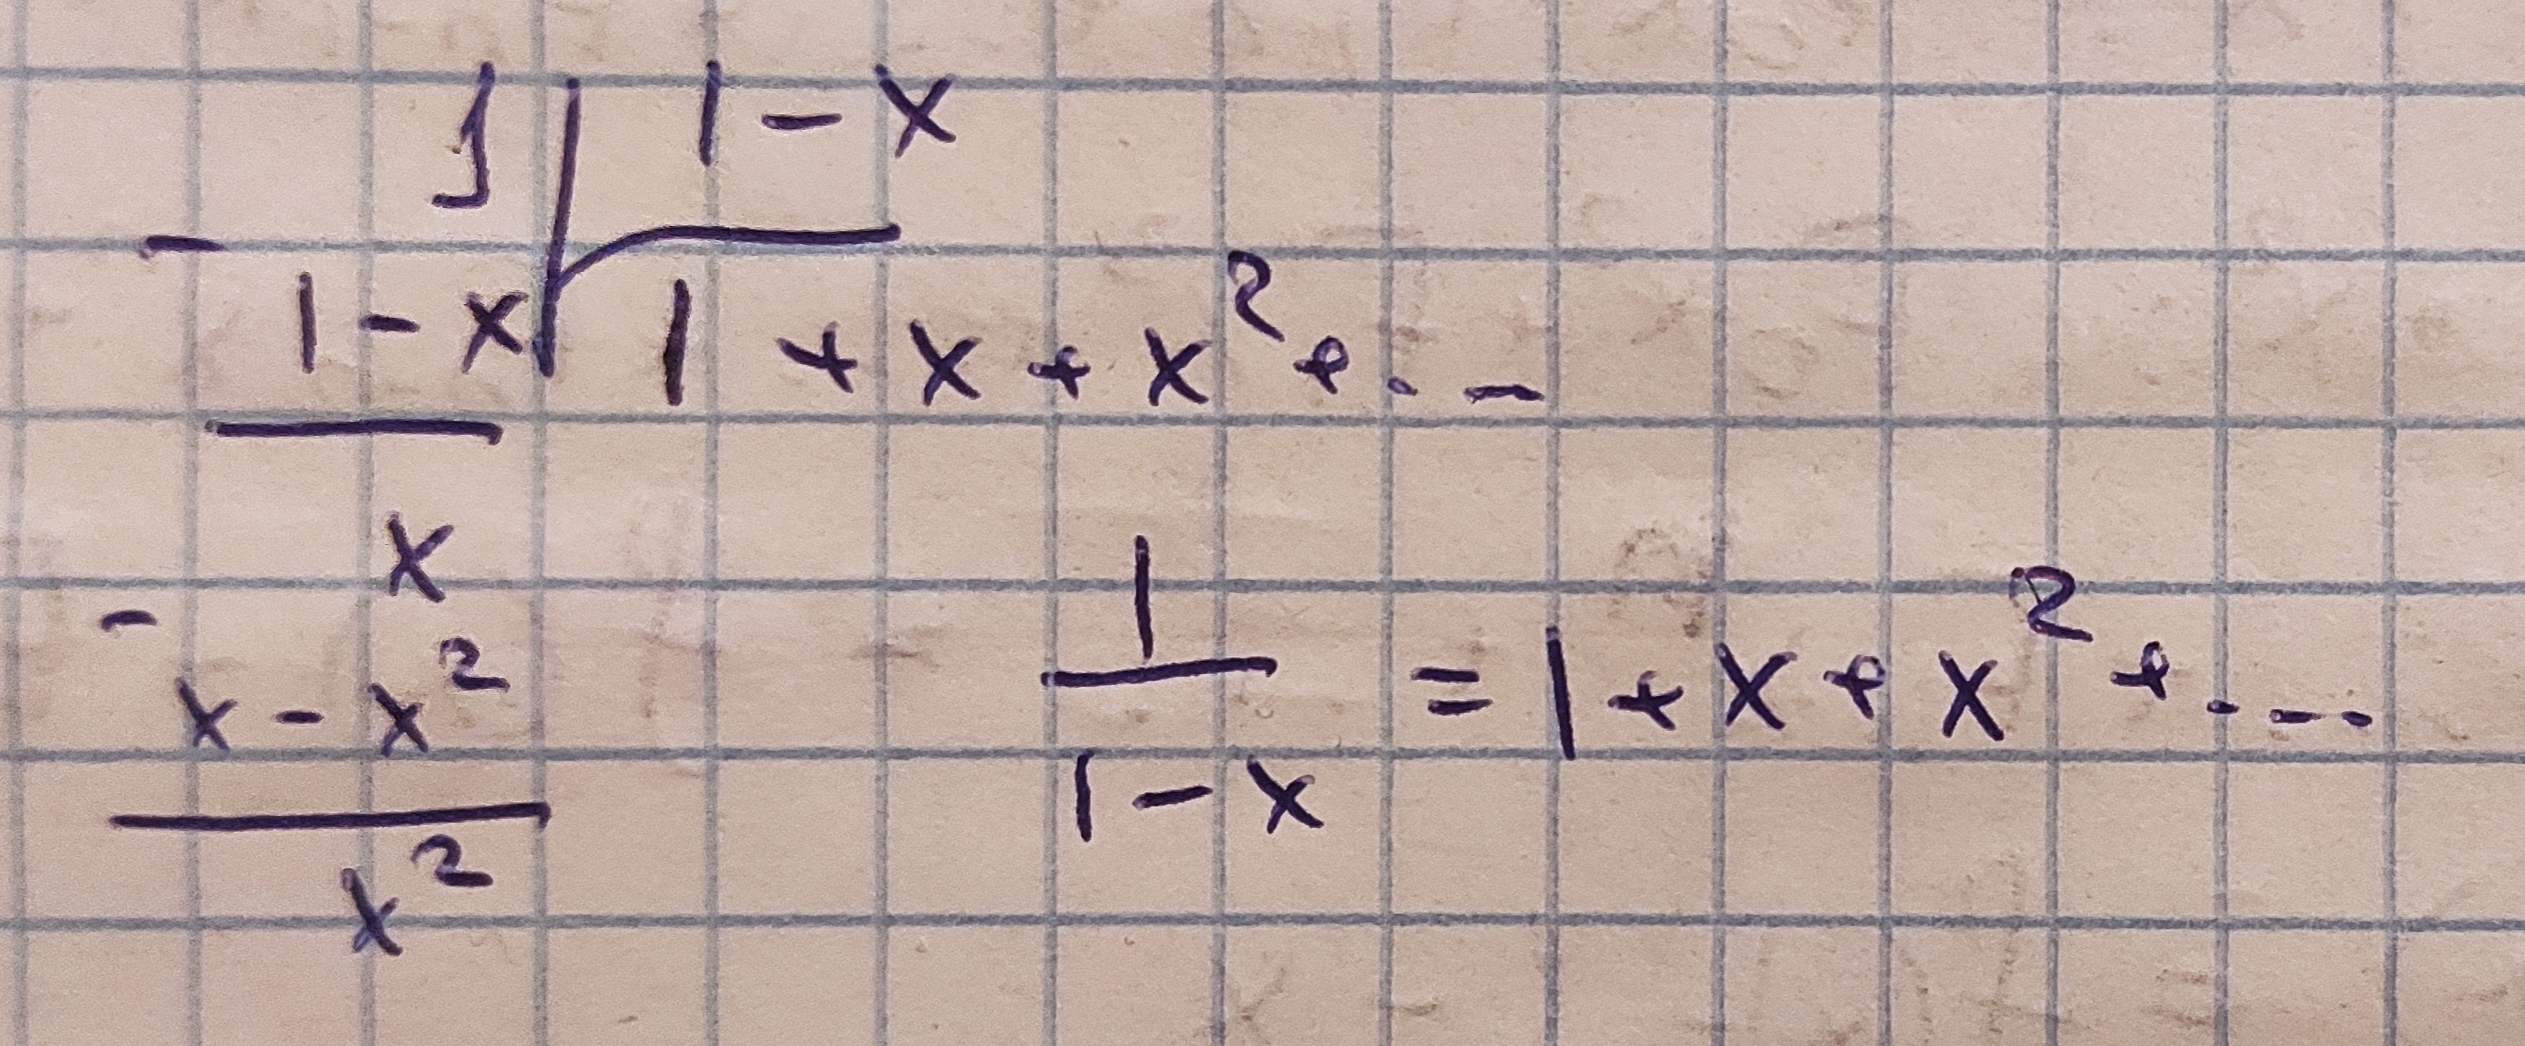
\includegraphics[scale=0.1]{images/55.jpg}}
\end{figure}
\par
\subsection*{Комбинаторное тождество:} 
$$\left(\frac{1}{1-x^2}\right)^2=\left(\frac{1}{1-x}\right)^2\left(\frac{1}{1+x}\right)^2$$
$$\left(\frac{1}{1-x}\right)^2=1+2x+3x^2+...+(n+1)x^n+... \mbox{ (см. билет 54)}$$
$$\left(\frac{1}{1+x}\right)^2=1-2x+3x^2-...+(-1)^n(n+1)x^n+...$$
\par Коэффициент исходного ряда при $x^n$, если мы считаем через произведение, равен:
$$1(n+1)(-1)^n+2n(-1)^{n-1}+...+(n+1)1(-1)^0=\sum_{k=0}^n (k+1)(n+1-k)(-1)^{n-k}$$
\par Посчитаем формулу исходного ряда через квадрат обратного ряда:
$$\left(\frac{1}{1-x^2}\right)^2=1+2x^2+3x^4+...+(n+1)x^{2n}$$
\par Таким образом, из равенства коэффициентов получаем тождество
$$\sum_{k=0}^n (k+1)(n+1-k)(-1)^{n-k} = \left\{
\begin{array}{ccc}
0, \mbox{ если } n=2l+1\\
l+1, \mbox{ если } n=2l\\
\end{array}
\right. $$

\subsection*{Строгое формальное определение формального степенного ряда через последовательности. Пример вычисления суммы и произведения рядов}
\par Рассмотрим множество последовательностей $(a_0, a_1, ..., a_n, ...)$ (здесь $a_i$ берутся из множества
чисел $\mathbb{Q}$, $\mathbb{R}$ или $\mathbb{C}$) и введём на них операции сложения и умножения следующим образом:
$$(a_0, a_1, . . .) + (b_0, b_1, . . .) = (a_0 + b_0, a_1 + b_1, . . .);$$
$$(a_0, a_1, . . .) · (b_0, b_1, . . .) = (c_0, c_1, . . .),\mbox{ где } c_n =\sum\limits_{j=0}^n a_j b_{n-j}$$
\par Выражения $a_0 \cdot 1+a_1 \cdot t+a_2 \cdot t^2+. . .+a_n \cdot t^n+. . .$ (с введёнными операциями сложения и умножения) называют \textbf{формальными степенными рядами}. $a_0$ называют свободным членом ряда.
\subsection*{Пример вычисления суммы и произведения рядов (задача 14.3):}
\begin{enumerate}
    \item $F = 1 + t + t^2 + . . ., G = 1 - t + t^2 - t^3 + . . .. $
    $$F + G=(1, 1, ...) + (1, -1, 1, ...) = (2, 0, 2, 0, ...)$$
    $$F \cdot G=(1, 1, ...)(1, -1, 1, ...)=(1, 1-1, 1-1+1, ..., \sum\limits_{i=1}^n g_i, ...)=(1, 0, 1, 0,...) $$
    \item $F =\sum\limits_{k=0}^{\infty} \frac{1}{k!}t^k, \; G =\sum\limits_{k=0}^{\infty} \frac{(-1)^k}{k!}t^k$
    $$F \cdot G: \; c_n=\sum\limits_{k=0}^n \frac{(-1)^k}{k!(n-k)!}=\sum\limits_{k=0}^n \frac{(-1)^k}{n!} C_n^k=\left\{
\begin{array}{ccc}
\frac{1}{n!}=1, \mbox{ если } n=0\\
0, \mbox{ если } n \geq 1\\
\end{array}
\right. \mbox{(из знакопеременной суммы см. билет 32)}$$
$$F \cdot G = (1, 0, 0, ...)=1$$
$$F^2: \; c_n=\sum\limits_{k=0}^n \frac{1}{k!(n-k)!}=\frac{1}{n!} \sum\limits_{k=0}^n C_n^k=\frac{2^n}{n!} \mbox{ (из комбинаторного тождества)}$$
$$F^2=\sum\limits_{k=0}^{\infty} \frac{1}{k!}(2t)^k$$
\end{enumerate}